\subsection{Elektronische mail op het internet}

3 componenten: \textbf{user agents} (Outlook, Thunderbird, ...), \textbf{mailservers} en \textbf{SMTP}.

\subsubsection{Mail Servers}

\textbf{Mailbox}: contains incoming messages for user
\textbf{message queue} of outgoing (to be sent) mail messages
\textbf{SMTP protocol} between mail servers to send email messages
\begin{itemize}
    \item client: sending mail server
    \item “server”: receiving mail server
\end{itemize}

\subsubsection{SMTP}

\begin{figure}[h]
\centering
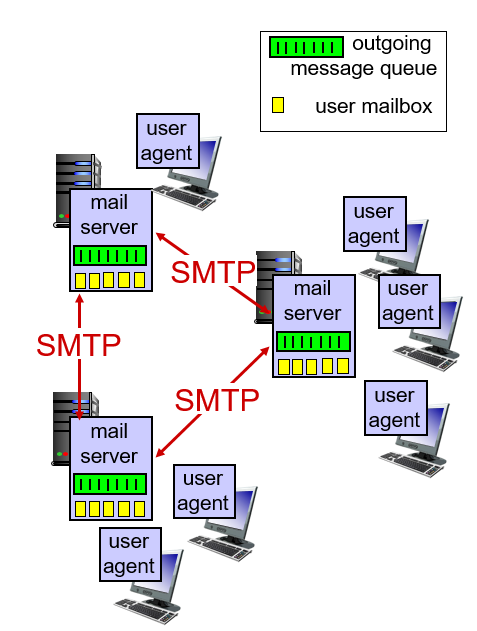
\includegraphics[height=3in]{./img/imghfdst2/hdst2puntje8.png}
\caption{Voorbeeld van een smtp }
\label{fig:smtp}
\end{figure}


\bi
\itf uses TCP to reliably transfer email message from client to server, port 25
\itf direct transfer: sending server to receiving server
\itf three phases of transfer
    \bi
    \itf handshaking (greeting)
    \itf transfer of messages
    \itf closure
    \ei
\itf command/response interaction (like HTTP, FTP)
    \bi
    \itf commands: ASCII tekst
    \itf response: status code and phrase
    \ei
\itf messages must be in 7-bit ASCI
\ei
\noindent Belangrijk:
\bi
\itf SMTP uses persistent connections
\itf SMTP requires message (header \& body) to be in 7-bit ASCII
\itf SMTP server uses CRLF.CRLF to determine end of message
\ei

\noindent Veronderstel dat Alice een simpele ASCII bericht naar Bob wilt sturen:

\begin{enumerate}
 \item Alice roept haar user agent op, voorziet Bob zijn email adres, stelt een bericht op en beveelt dan de user agent om het bericht te sturen.
 \item Alice haar user agent zend het bericht naar de mail server waar het in de message queue geplaatst wordt.
 \item De client kant van SMTP, ziet het bericht in de message queue. Het opent een TCP connectie naar een SMTP server, die op Bob zijn mail server runt.
 \item Na een paar initiële SMTP handshaking, zend de SMTP client Alice haar bericht in de TCP connectie.
 \item Bij Bob zijn mail server, de server kant van SMTP krijgt het bericht. Bob zijn mail server plaatst dan het bericht in Bob zijn mailbox.
 \item Bob roept zijn user agent op om het bericht te lezen.
\end{enumerate}
Normaal gezien gebruikt SMTP geen tussenliggende mail server voor het zenden van mails.

\begin{figure}[h]
\centering
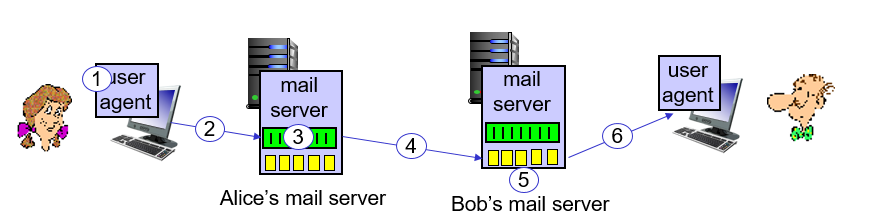
\includegraphics[width=3in]{./img/imghfdst2/hdst2puntje9.png}
\caption{Voorbeeld van een verbinding }
\label{fig:verbinding}
\end{figure}

\subsubsection{Vergelijking met HTTP}


\bi
\itf HTTP \textbf{kopieert} bestanden/SMTP \textbf{verwisselt} bestanden \textbf{uit}
\itf \textbf{HTTP} is een \textbf{pullprotocol}: Iemand plaats informatie op een server en gebruikers ‘trekken’ de informatie er van af.
\itf HTTP stuurt elk object in een \textbf{apart} antwoordbericht
\itf SMTP stuurt alle objecten in 1 bericht bestaande uit meerdere delen (= \textbf{multipart message})
\itf SMTP is een \textbf{pushprotocol}: de mails worden ‘doorgeduwd’
\itf SMTP werkt alleen wanneer elk bericht bestaat uit 7 bit-ASCII-tekst
\ei

\clearpage

\subsubsection{Mail bericht formaten}

\begin{figure}[h]
\centering
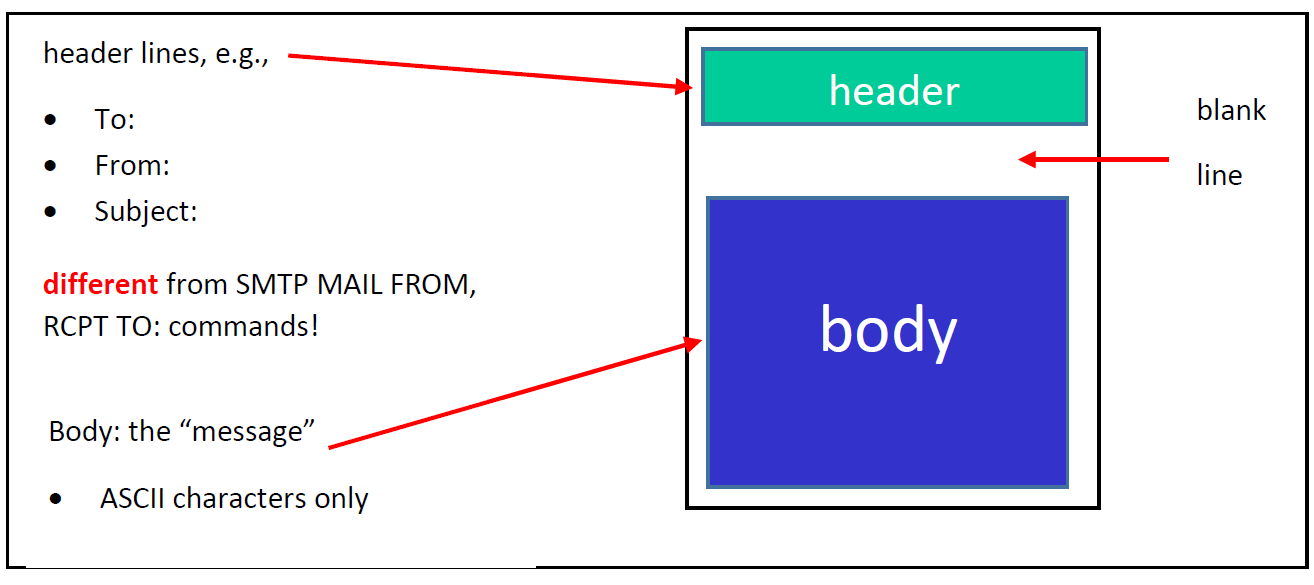
\includegraphics[width=3in]{./img/imghfdst2/formatmail.PNG}
\caption{Voorbeeld van een format mail }
\label{fig:format mail}
\end{figure}

\noindent Elke header moet een From:, To: en Subject: header line bevatten. Het is belangrijk om op te merken dat deze header line verschillend zijn van de SMTP commando’s. Na de bericht header volgt er een lege lijn, en dan het bericht in ASCII.

\subsubsection{Mail toegang protocollen}

\begin{figure}[h]
\centering
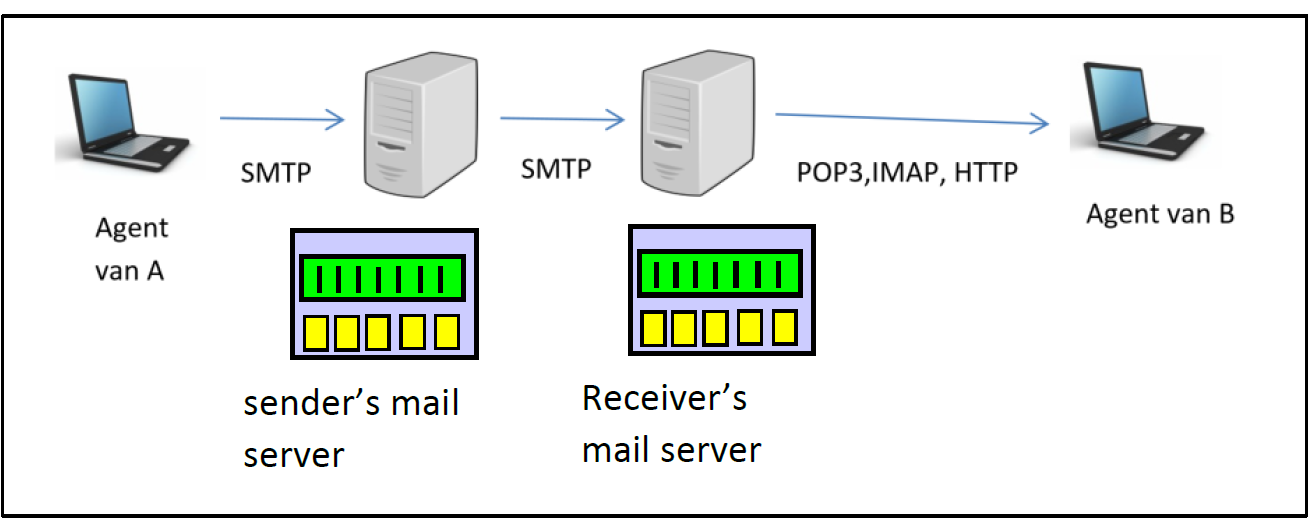
\includegraphics[width=3in]{./img/imghfdst2/access.PNG}
\caption{Voorbeeld van een pullprotocol }
\label{fig:pullprotocol}
\end{figure}

\noindent Aangezien SMTP een \textbf{pushprotocol} is, kan men via SMTP \textbf{geen} mails halen van de mailserver, hiervoor zijn er andere protocollen, namelijk: \textbf{POP3, IMAP en HTTP.}

\noindent Deze protocollen zijn dus \textbf{pullprotocollen} die worden gebruikt om mails van de mailserver te halen.

%\clearpage

\subsubsubsection{POP3 = Post Office Protocol}

3 fasen:
\be
\itf \textbf{Autorisatiefase}: User Agent verzendt de gebruikersnaam en wachtwoord naar de mailserver
\itf \textbf{Transactiefase}: De berichten worden opgehaald uit de mailserver. Tijdens deze fase is het mogelijk om andere berichten te markeren.
\itf \textbf{Updatefase}: Begint wanneer de cliënt de opdracht ‘QUIT’ heeft gegeven. Op dat moment verwijdert de mailserver alle berichten die gemarkeerd zijn met ‘verwijderen’.
\ee

\noindent Bij POP3 wordt er steeds gewerkt met een opdracht/antwoord-gang van zaken. Er zijn 2 mogelijke antwoorden die de mailserver kan sturen:
\bi
\itf +OK: De opdracht werd correct uitgevoerd
\itf -ERR: Er is een fout opgetreden.
\ei

\noindent Er wordt geen statusinformatie bijgehouden over de POP3-sessies = stukken eenvoudiger.

\subsubsubsection{IMAP = Internet Mail Access Protocol}

IMAP biedt de mogelijkheid om op de server mappen te maken en de mails te categoriseren + houdt sessie-informatie bij.

\bi
\itf keeps all messages in one place: at server
\itf allows user to organize messages in folders
\itf keeps user state across sessions:
\bi
\itf names of folders and mappings between message IDs and folder name
\ei
\ei

\subsubsubsection{Web gebaseerde E-mail}

Meer en meer gebruikers verzenden en bereiken hun e-mail via hun web browsers. Met deze service, is de user agent een ordinaire web browser, en de gebruiker communiceert met zijn remote mailbox door HTTP. Wanneer een ontvanger zijn berichten in zijn mailbox wilt zien, is het email bericht die verstuurt wordt van Bob zijn mail server naar Bob zijn browser gebruik makend van het HTTP protocol in plaats van het POP3 of IMAP protocol.
